% =============================================================================
% Lecture 10: Bayesian Statistics I — Foundations
% ECON 8310: Business Forecasting
% University of Nebraska at Omaha
% =============================================================================

\documentclass[aspectratio=169, 11pt]{beamer}

\input{header}

% ---- Lecture metadata --------------------------------------------------------
\title[Bayesian I: Foundations]{Bayesian Statistics I: Foundations}
\subtitle{ECON 8310: Business Forecasting --- Lecture 10}
\author{Department of Economics}
\institute{University of Nebraska at Omaha}

% =============================================================================
\begin{document}
% =============================================================================

\begin{frame}
  \titlepage
\end{frame}

% ---- Outline ----------------------------------------------------------------
\begin{frame}{Lecture Outline}
  \tableofcontents
\end{frame}

% =============================================================================
\section{Why Bayesian Thinking?}
% =============================================================================

\sectionslide{Why Bayesian Thinking?}{%
  A different answer to the question of what a forecast should tell you.}

% --- Slide: frequentist vs bayesian ------------------------------------------
\begin{frame}{Frequentist vs.\ Bayesian: What Is Random?}
  The whole difference is which thing you treat as uncertain.

  \vspace{0.1cm}
  \begin{center}
    {\small
    \begin{tabular}{p{2.2cm}p{4.9cm}p{5.0cm}}
      \toprule
       & \textbf{Frequentist} & \textbf{Bayesian} \\
      \midrule
      The parameter & A fixed, unknown constant & A quantity you are uncertain about \\[3pt]
      The data & Random --- one draw of many possible samples & Fixed --- it is what you observed \\[3pt]
      The answer & A point estimate and a standard error & A full distribution over values \\[3pt]
      Prior belief & No formal place for it & Stated explicitly, and updated \\
      \bottomrule
    \end{tabular}
    }
  \end{center}

  \vspace{0.1cm}
  Everything else follows from that first row. If the parameter is fixed, you can only describe
  how your \emph{estimate} would vary across hypothetical repeated samples. If the parameter is
  uncertain, you can describe your uncertainty about \emph{it} directly --- which is almost
  always the question someone actually asked.
\end{frame}

% --- Slide: what a posterior buys --------------------------------------------
\begin{frame}{What This Buys You in a Meeting}
  A 95\% \textbf{confidence} interval of $[0.02,\ 0.08]$ does \emph{not} mean a 95\% chance the
  parameter is in it. It means the \emph{procedure} catches the true value in 95\% of repeated
  samples.

  \vspace{0.15cm}
  A 95\% \textbf{credible} interval \emph{does} mean that, given your model and data.

  \begin{keybox}
    One you can say to a decision-maker; the other you keep correcting.
  \end{keybox}

  \vspace{0.1cm}
  A full distribution also answers a planner's question: \emph{what is the chance we stock out
  if we order 400 units?}

  \vspace{0.1cm}
  \muted{\footnotesize\itshape The cost: you must state a prior, and defend it.}
\end{frame}

% =============================================================================
\section{Bayes' Theorem}
% =============================================================================

\sectionslide{Bayes' Theorem}{%
  One equation, and it is a bookkeeping rule rather than a philosophy.}

% --- Slide: Bayes' theorem ---------------------------------------------------
\begin{frame}{Bayes' Theorem \parencite{Gelman2013}}
  \begin{definitionbox}{The update rule}
    \[
      \underbrace{p(\theta \mid \mathcal{D})}_{\text{posterior}}
      = \frac{\overbrace{p(\mathcal{D} \mid \theta)}^{\text{likelihood}}
              \cdot \overbrace{p(\theta)}^{\text{prior}}}
             {\underbrace{p(\mathcal{D})}_{\text{evidence}}}
    \]
  \end{definitionbox}

  Read it as a sentence. \textbf{What I believe after seeing the data} equals \textbf{how well
  each value explains the data}, times \textbf{what I believed beforehand}, rescaled to sum to one.

  \vspace{0.1cm}
  The denominator is only that rescaling --- it does not change the \emph{shape}. So the working
  form is:
  \[
    \text{posterior} \;\propto\; \text{likelihood} \times \text{prior}
  \]
  \vspace{-0.3cm}

  \textbf{You will not compute this by hand}, and this course never asks you to. You are
  responsible for choosing the prior, checking the sampler worked, and reading the posterior.
\end{frame}

% --- Slide: the update, graphically ------------------------------------------
\begin{frame}{The Update, in Pictures}
  A conversion rate $\theta$: a $\text{Beta}(5, 45)$ prior, then 30 successes in 200 trials.
  \begin{center}
    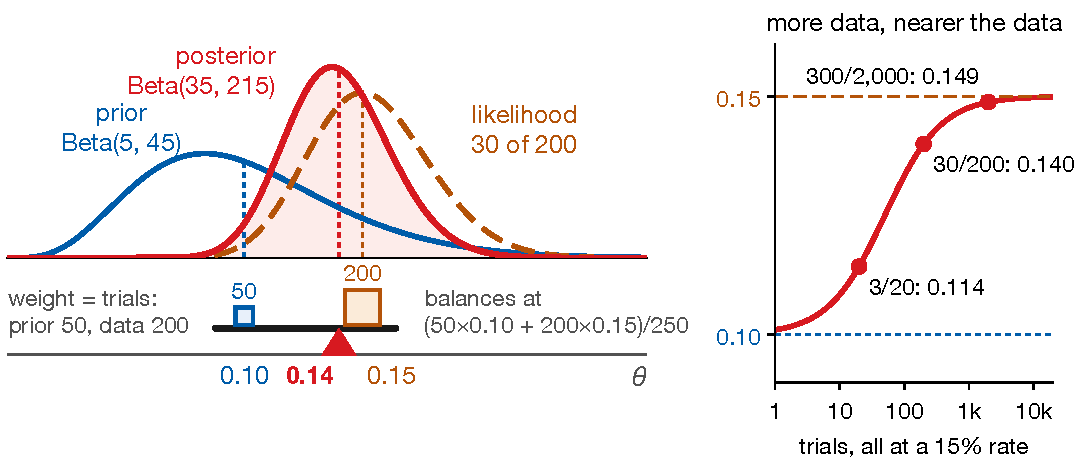
\includegraphics[height=4.8cm]{../Figures/Lecture10_BayesianFoundations/bayes_update.pdf}
  \end{center}
  \vspace{-0.3cm}
  {\small Multiply the curves point by point and rescale: the posterior sits between them. Its
  mean balances the prior's 0.10, worth 50 observations, against the data's 0.15, worth 200, at
  \textbf{0.14}. With little data the prior does most of the work: a feature when it is
  defensible, a problem when it is not.}
\end{frame}

% =============================================================================
\section{Prior Distributions}
% =============================================================================

\sectionslide{Prior Distributions}{%
  The part you have to justify, and the part people worry about.}

% --- Slide: common priors ----------------------------------------------------
\begin{frame}{Priors You Will Actually Use}
  A prior is a distribution over a parameter, chosen to match what that parameter \emph{can} be.
  \begin{center}
    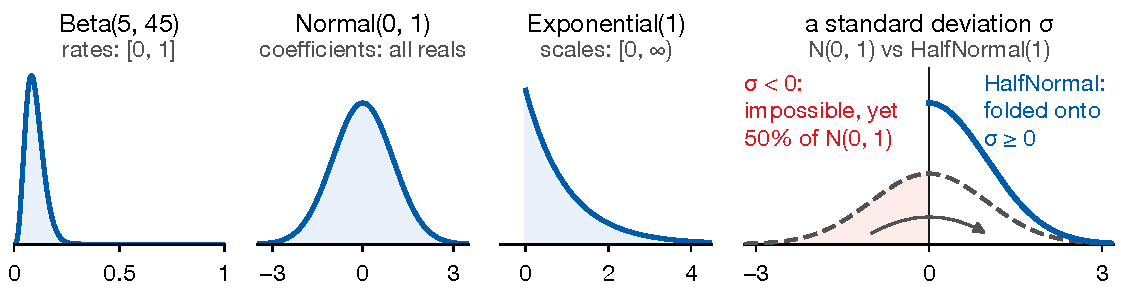
\includegraphics[width=\textwidth]{../Figures/Lecture10_BayesianFoundations/priors_support.pdf}
  \end{center}
  \vspace{-0.2cm}
  \textbf{The support is the first thing to get right.} A Normal prior on a standard deviation
  puts half its mass on negative values, which are impossible: the model is not wrong so much as
  incoherent. Fold that half onto $\sigma \ge 0$ and you have the HalfNormal.
\end{frame}

% --- Slide: choosing a defensible prior --------------------------------------
\begin{frame}{Choosing a Prior You Can Defend}
  The standard objection to Bayesian work is that the prior is arbitrary. The standard answer is
  that you should not be choosing arbitrary priors.

  \begin{center}
    {\small
    \begin{tabular}{p{3.3cm}p{9.0cm}}
      \toprule
      \textbf{Weakly informative} & Rules out the absurd, stays agnostic about the plausible. A
      Normal(0, 1) on a standardized coefficient says ``probably not larger than about 2,''
      which is nearly always true and nearly never controversial. \textbf{This is the default.} \\[3pt]
      \textbf{Informative} & Encodes real prior evidence --- last year's conversion rate, a
      published elasticity. Defensible when you can name the source. \\[3pt]
      \textbf{Flat / ``uninformative''} & Sounds neutral, often is not, and can be improper.
      Avoid it as a reflex choice. \\
      \bottomrule
    \end{tabular}
    }
  \end{center}

  \textbf{The honest framing:} a prior is an assumption stated in public, where it can be argued
  with. Frequentist analyses contain assumptions too --- functional form, variable selection,
  sampling scheme --- they are just not written as distributions.
\end{frame}

% =============================================================================
\section{Posterior Inference with PyMC}
% =============================================================================

\sectionslide{Posterior Inference with PyMC}{%
  Sampling, the code, and how to tell whether the answer is trustworthy.}

% --- Slide: MCMC -------------------------------------------------------------
\begin{frame}{MCMC: The Big Idea}
  Beyond textbook examples, the denominator $p(\mathcal{D})$ cannot be computed. So we do not
  compute the posterior: we \textbf{draw samples from it}.
  \begin{center}
    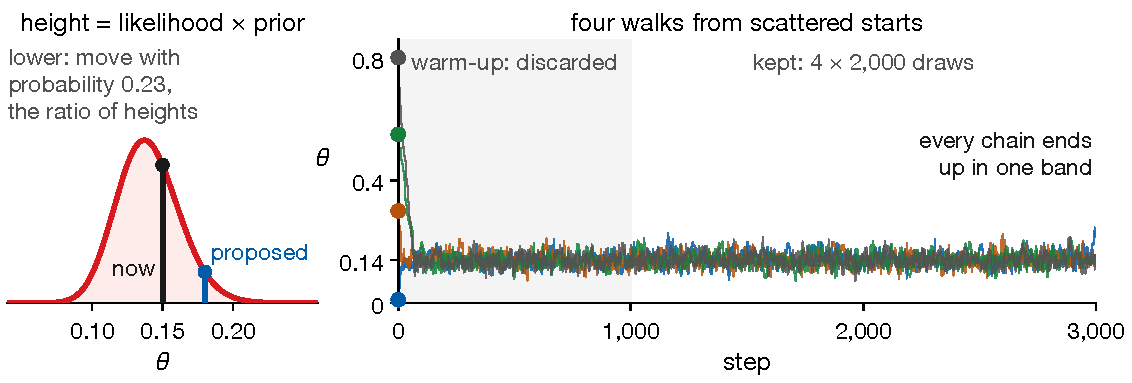
\includegraphics[height=4.4cm]{../Figures/Lecture10_BayesianFoundations/mcmc_walk.pdf}
  \end{center}
  \vspace{-0.25cm}
  {\small Each step compares two heights of likelihood $\times$ prior: higher, move; lower, move
  with probability equal to their ratio. Both heights carry the same $p(\mathcal{D})$, so it
  cancels.}

  \muted{\footnotesize\itshape This is random-walk Metropolis. PyMC's default, NUTS, takes smarter
  steps; the intuition is unchanged.}
\end{frame}

% --- Slide: the samples are the answer ----------------------------------------
\begin{frame}{The Samples Are the Answer}
  The record of where you walked \emph{is} the answer: a histogram of the kept draws has the shape
  of the posterior, and nobody ever computed it.
  \begin{center}
    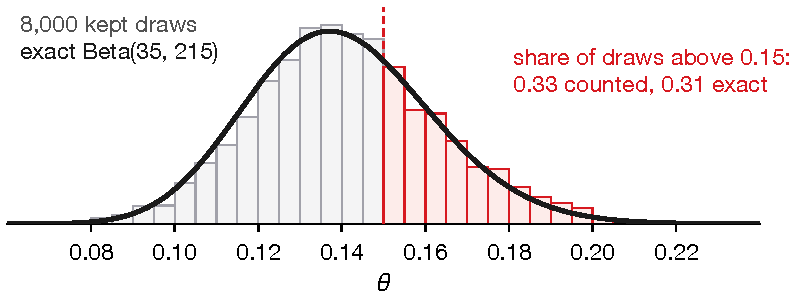
\includegraphics[height=3.4cm]{../Figures/Lecture10_BayesianFoundations/mcmc_histogram.pdf}
  \end{center}
  \vspace{-0.3cm}
  \begin{keybox}
    \textbf{Every summary is a count.} Posterior mean, credible interval, the probability of any
    event: each is counted from the draws, not derived.
  \end{keybox}
  The planner's stock-out question becomes one line: the share of simulated demand draws above
  400 units.
\end{frame}

% --- Slide: PyMC first model -------------------------------------------------
\begin{frame}{PyMC: A First Model}
  \begin{examplebox}{Estimating a conversion rate --- 30 successes in 200 trials}
    {\tiny\linespread{1.2}\selectfont
    \texttt{import pymc as pm}\\[2pt]
    \texttt{with pm.Model() as model:}\\
    \texttt{\mbox{}\ \ \ \ theta = pm.Beta("theta", alpha=5, beta=45)\ \ \ \ \ \ \ \# prior}\\
    \texttt{\mbox{}\ \ \ \ obs\ \ = pm.Binomial("obs", n=200, p=theta,\ \ \ \ \ \ \ \# likelihood}\\
    \texttt{\mbox{}\ \ \ \ \ \ \ \ \ \ \ \ \ \ \ \ \ \ \ \ \ \ \ \ observed=30)}\\
    \texttt{\mbox{}\ \ \ \ idata = pm.sample(2000, tune=1000, chains=4, random\_seed=42)}\\[3pt]
    \texttt{import arviz as az}\\
    \texttt{az.plot\_posterior(idata)}
    }
  \end{examplebox}
  A PyMC model describes \textbf{how the data could have been generated}: what I believe about
  the rate, and how observations arise given it. You write the story; the sampler infers.

  \texttt{tune=1000} discards the first 1{,}000 steps, while the sampler is still finding the
  high ground. \texttt{chains=4} runs four independent walks --- which is what makes the next
  slide possible.
\end{frame}

% --- Slide: diagnostics ------------------------------------------------------
\begin{frame}{Did the Sampler Actually Work? \parencite{MartinKumarLao2021}}
  MCMC can fail quietly. It always returns samples; whether they came from the posterior is a
  separate question.
  \begin{center}
    {\small
    \begin{tabular}{p{2.5cm}p{3.0cm}p{6.6cm}}
      \toprule
      \textbf{Check} & \textbf{Want} & \textbf{What it means} \\
      \midrule
      $\hat{R}$ & $< 1.01$ & Did the chains land in the same place? If not, nothing else
      matters. \\[2pt]
      ESS & $> 400$ & Effective sample size --- 8{,}000 correlated draws may carry as much
      information as 200 independent ones. \\[2pt]
      Divergences & $0$ & The sampler hit terrain it could not navigate. Even a few means the
      posterior is explored wrongly. \\
      \bottomrule
    \end{tabular}
    }
  \end{center}

  \texttt{az.summary(idata, ci\_kind="hdi", ci\_prob=0.94)} prints the interval, $\hat{R}$ and ESS.
  \textbf{Pass both arguments} --- ArviZ now defaults to an 89\% equal-tailed interval, not the HDI.

  On the model above: $\hat{R} = 1.00$, ESS 3{,}290, zero divergences. \textbf{Report all three.}
\end{frame}

% --- Slide: prior predictive checks -----------------------------------------
\begin{frame}{Prior Predictive Checks \parencite{McElreath2020}}
  Before touching the data, simulate from the prior alone.

  \begin{examplebox}{Two lines}
    {\scriptsize\linespread{1.0}\selectfont
    \texttt{with model:}\\
    \texttt{\mbox{}\ \ \ \ prior\_pred = pm.sample\_prior\_predictive(500)}\\[2pt]
    \texttt{az.plot\_ppc(prior\_pred, group="prior")}
    }
  \end{examplebox}

  \textbf{Ask whether the simulated data could plausibly have come from your business.}
  Impossible values --- negative sales, probabilities above one --- mean the prior is
  misspecified, not merely wide.

  \begin{keybox}
    A prior predictive check is \textbf{model debugging} that costs two lines --- and the habit
    most often skipped.
  \end{keybox}
\end{frame}

% --- Slide: three priors, three predictions ----------------------------------
\begin{frame}{Three Priors, Three Predictions}
  The conversion-rate model before any data: successes out of 200 under each prior.
  \begin{center}
    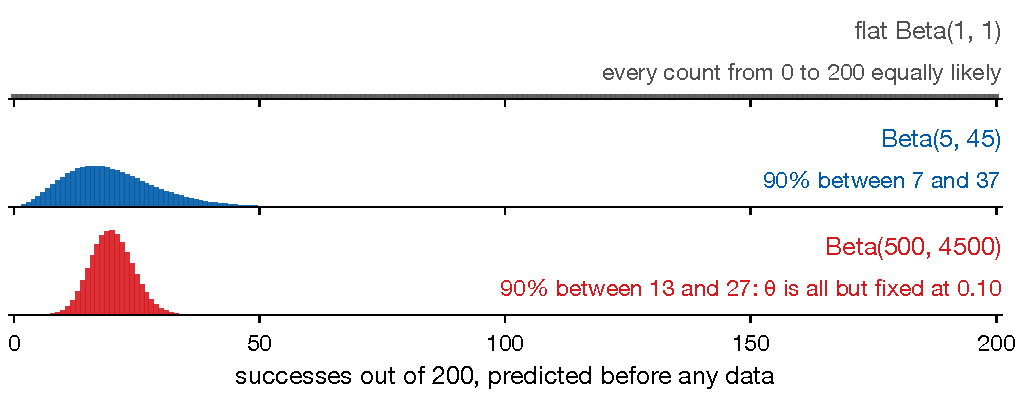
\includegraphics[height=4.4cm]{../Figures/Lecture10_BayesianFoundations/prior_predictive.pdf}
  \end{center}
  \vspace{-0.25cm}
  {\small \textbf{Flat} is too vague: 190 successes is as likely as 20. \textbf{Beta(500, 4500)}
  is too tight: worth 5{,}000 observations, it has fixed $\theta$ before the data arrive, and the
  spread left is binomial noise. \textbf{Beta(5, 45)} rules out the absurd and leaves room.}
\end{frame}

% =============================================================================
\section{Key Takeaways}
% =============================================================================

\sectionslide{Key Takeaways}{%
  Bayesian inference: beliefs in, beliefs out.
  Data updates your prior into a posterior.}

% --- Slide: Key takeaways ---------------------------------------------------
\begin{frame}{Lecture 10: Key Takeaways}
  \begin{keybox}
    {\small
    \begin{enumerate}
      \item \textbf{Bayesian inference}: the posterior $p(\theta \mid \mathcal{D})$ is what you
            believe after the data.
      \item \textbf{Bayes' theorem}: posterior $\propto$ likelihood $\times$ prior, landing
            between the two, nearer the weightier.
      \item \textbf{Priors:} match the support first; weakly informative by default.
      \item \textbf{MCMC} (NUTS in PyMC) draws samples; every summary is counted from them.
      \item \textbf{Check before you trust}: $\hat{R}$, ESS and divergences, and a prior
            predictive check, every time.
    \end{enumerate}
    }
  \end{keybox}
  \muted{\itshape Next: Bayesian Statistics II ---
  Bayesian time series models, trend and seasonality, hierarchical models.}
\end{frame}

% --- References ---------------------------------------------------------------
\begin{frame}[allowframebreaks]{References}
  \printbibliography[heading=none]
\end{frame}

% =============================================================================
\end{document}
% =============================================================================
